\documentclass[]{paper}
\usepackage{graphicx}

% type user-defined commands here

\begin{document}

\title{FutureGrid 2012 Project Challenge} 
\author{Shantenu Jha 
  \and ...
}
\date{May 15th, 2012}
\maketitle

\begin{abstract}
\end{abstract}

\section{Introduction}
FutureGrid provides students and researchers with new possibilities to
engage in science relating to the state-of-the-art in cloud and grid computing.
As members of the RADICAL group, we have taken full advantage
of the opportunities that FutureGrid provides.  Here are some of the ways
we are using FutureGrid resources to push the envelope and pursue exciting
new discoveries.

\section{BigJob and BigData}

FutureGrid has been an important testbed for the development of 
BigJob~\cite{saga_bigjob_condor_cloud} and BigData~\cite{pstar-sc-2012,pmr-2012}.


\section{P* - Pilot-Job Interoperability}

Pilot-Jobs (PJ) have become one of the most successful abstractions in
distributed computing. In spite of extensive uptake, there does not exist a
well defined, unifying conceptual model of Pilot-Jobs, which can be used to
define, compare and contrast PJ implementations. This presents a barrier to
extensibility and interoperability. The P*
model~\cite{pstar-2012,pstar-sc-2012} provide a minimal but complete model of
Pilot-Jobs, which has been successfully applied to different Pilot-Job
frameworks, e.\,g.\ Condor and DIANE. The Pilot-API~\cite{pilot_api} provides 
an abstract, unified interface to PJ frameworks that adhere to the P* Model.

To demonstrated the interoperable and concurrent use of multiple Pilot-Job
frameworks via the Pilot-API on different production and research
infrastructures. Figure~\ref{fig:perf_perf-bfast-bj} shows how the Pilot-API
enables the user to run applications interoperably on different production and
research infrastructures. For this purpose we investigate the performance of
BFAST, a genome sequencing application. BFAST is very I/O sensitive -- we
observed for example, an I/O bottleneck if many BFAST CUs are run on the same
shared file system. The Pilot-API enables applications to scale to different
infrastructures in such cases.

\begin{figure}[t]
\centering
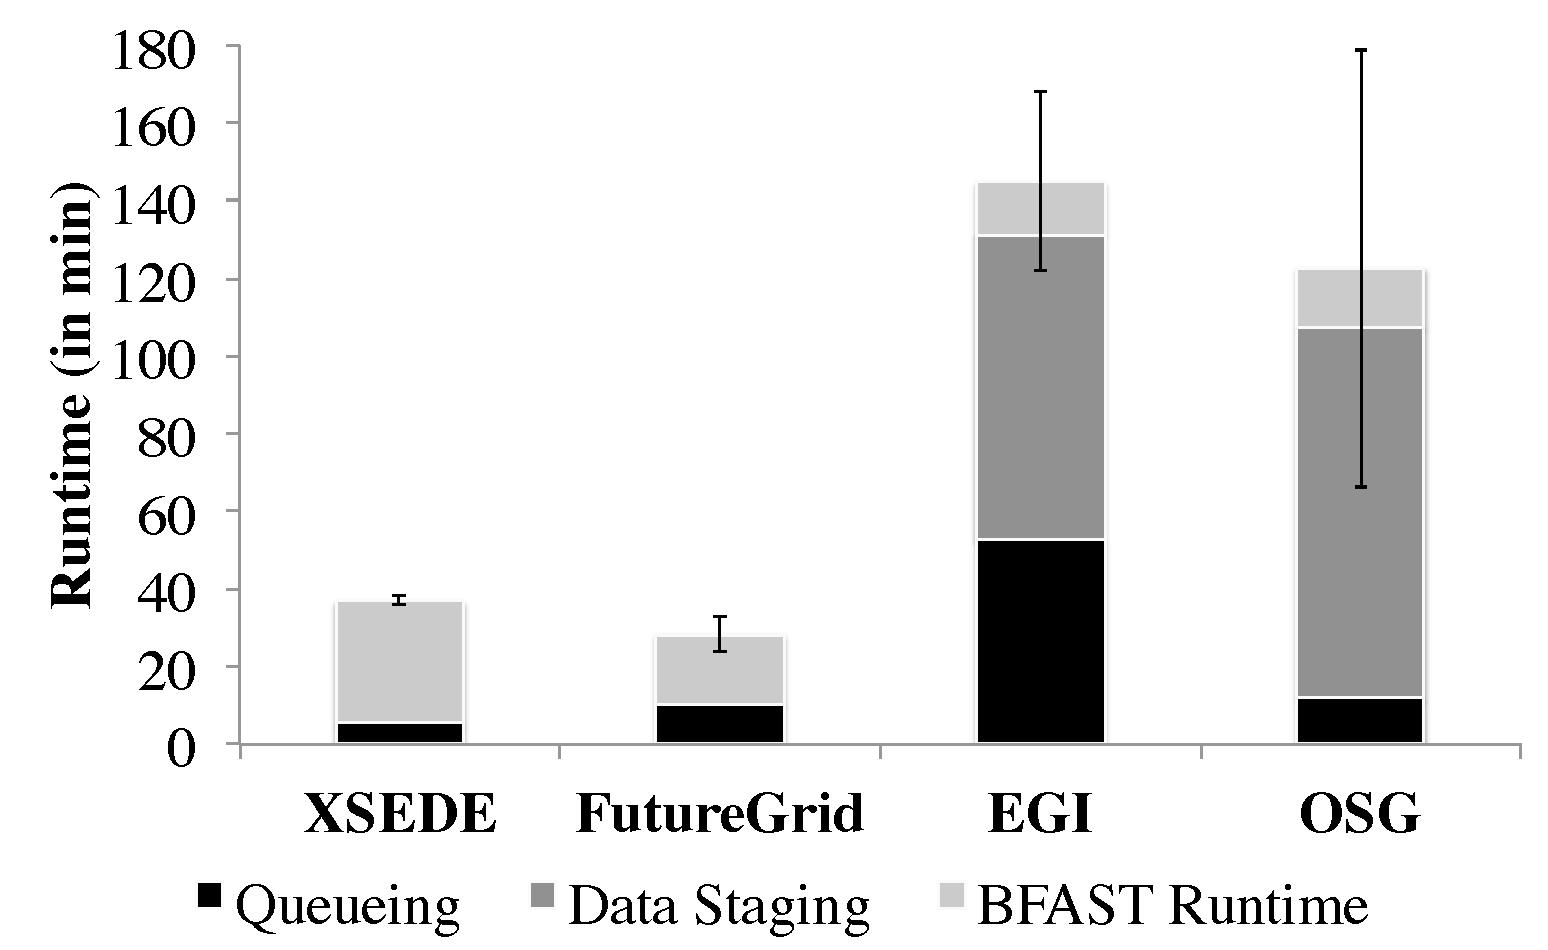
\includegraphics[width=0.7\textwidth]{figures/128-bfast-egi-fg-xsede-osg.pdf}
\caption{\textbf{PJ Framework Performance on XSEDE, FutureGrid, EGI and 
  OSG:} Running 128 BFAST match tasks on 128 cores. The longer runtimes on EGI 
  and OSG are mainly caused by  longer queuing times and the necessity to      
  stage all input files.}
  \label{fig:perf_perf-bfast-bj}
\end{figure}

% \begin{figure}[htbp]
% 	\centering
% 		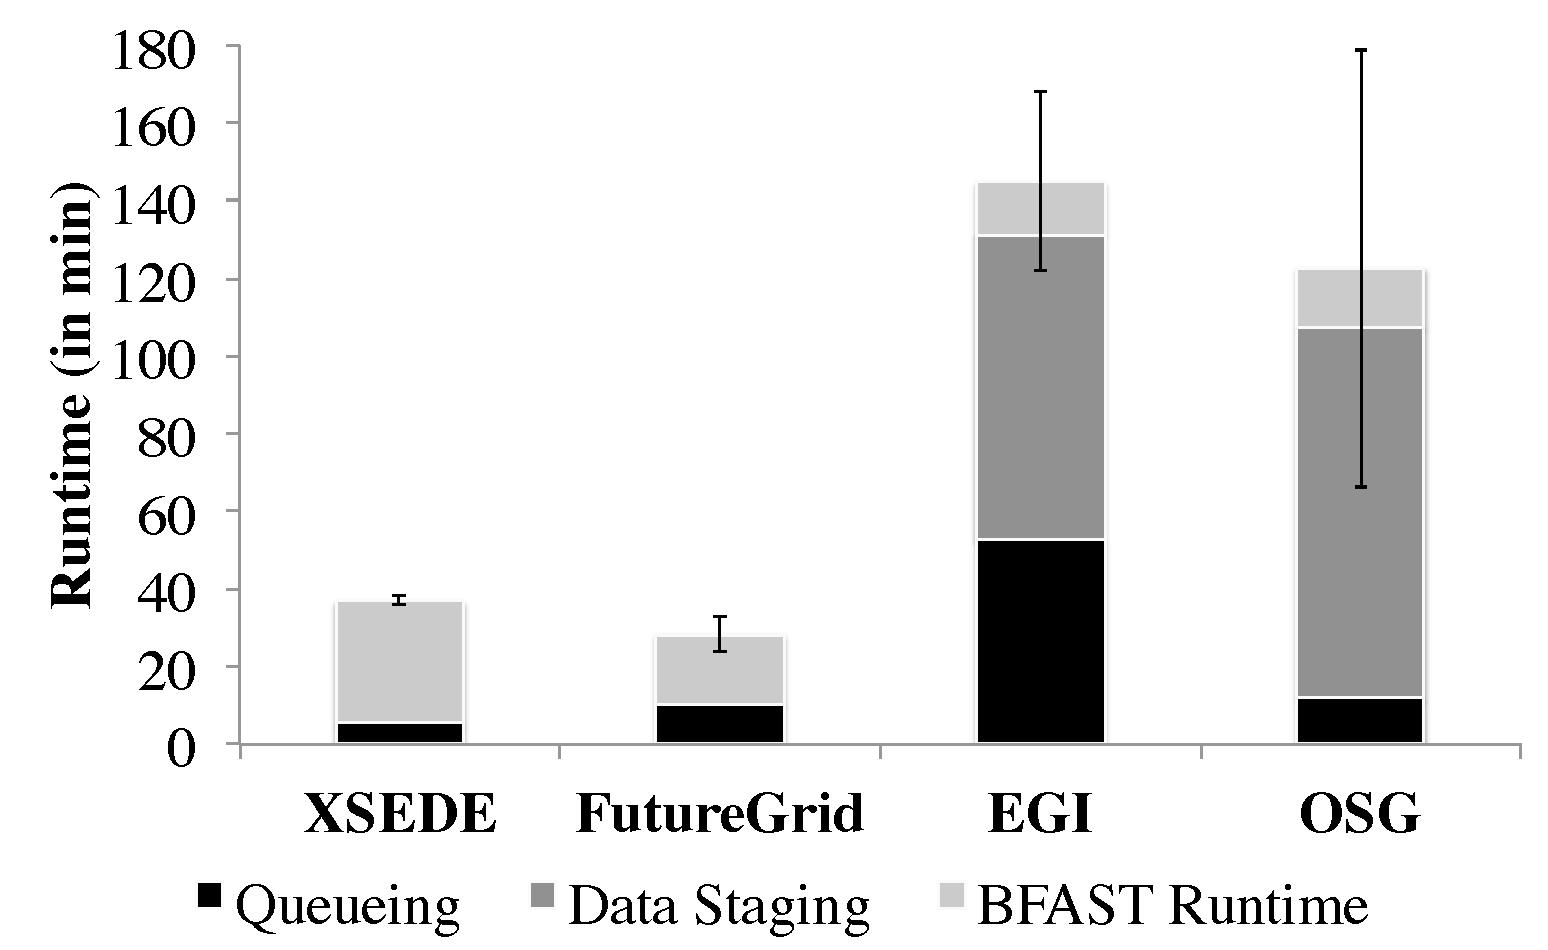
\includegraphics[height=3in]{figures/128-bfast-egi-fg-xsede-osg.pdf}
% 	\caption{caption}
% 	\label{fig:figures_128-bfast-egi-fg-xsede-osg}
% \end{figure}

\section{Replica Exchange}

Various applications have been developed using BigJob. An important 
application class are the application based on the replica-exchange algorithm.







\section{Conclusion}


\bibliographystyle{plain}
\bibliography{pilotjob,saga,saga-related}


\end{document}
